\begin{abstract}
  \setlength{\parskip}{1.5em}
  Surface-enhanced Raman spectroscopy can be used to enhance the Raman spectrum of graphene
  suspended on gold nanostructures. For basic studies it is desirable to convert the local
  electromagnetic field enhancement that can be simulated to the total
  enhancement that is measured in an experiment.

  This work presents a method to do this conversion using the software Lumerical~FDTD
  to simulate an experiment from ref.~\cite{heeg} and using 3D modelling software
  to simulate the geometry of the graphene layer within the experiment. Both sets of data
  are combined to calculate the local and total enhancement of the surface-enhanced
  Raman spectrum in the experiment.

  It will be shown that the projected electromagnetic field in the layer of graphene
  closely resembles the results of just using a planar slice at a height of \SI{40}{nm}
  which confirms the approximations used in ref.~\cite{heeg}. Taking laser
  geometry and spatial coherence in near-field Raman scattering into account, a
  total enhancement of $23.0$ is calculated which was measured as $12.8$ by ref.~\cite{heeg}.

  The presented method is exemplarily executed with the above-mentioned experiment
  but can be adapted for any Raman-active material suspended on nanostructures for
  surface-enhanced Raman spectroscopy.

  \begin{figure*}[!h]
    \centering
    \begin{subfigure}{0.48\textwidth}
      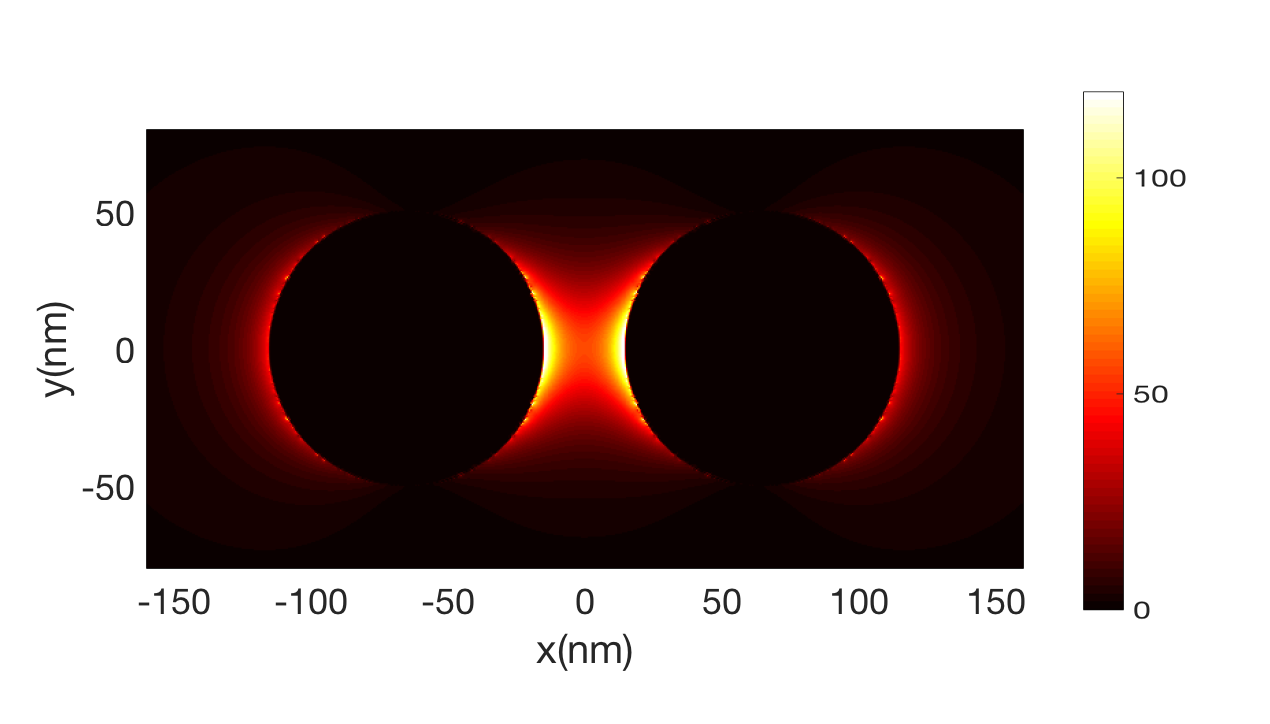
\includegraphics[width=\textwidth]{./images/40nm.png}
    \end{subfigure}
    \begin{subfigure}{0.48\textwidth}
      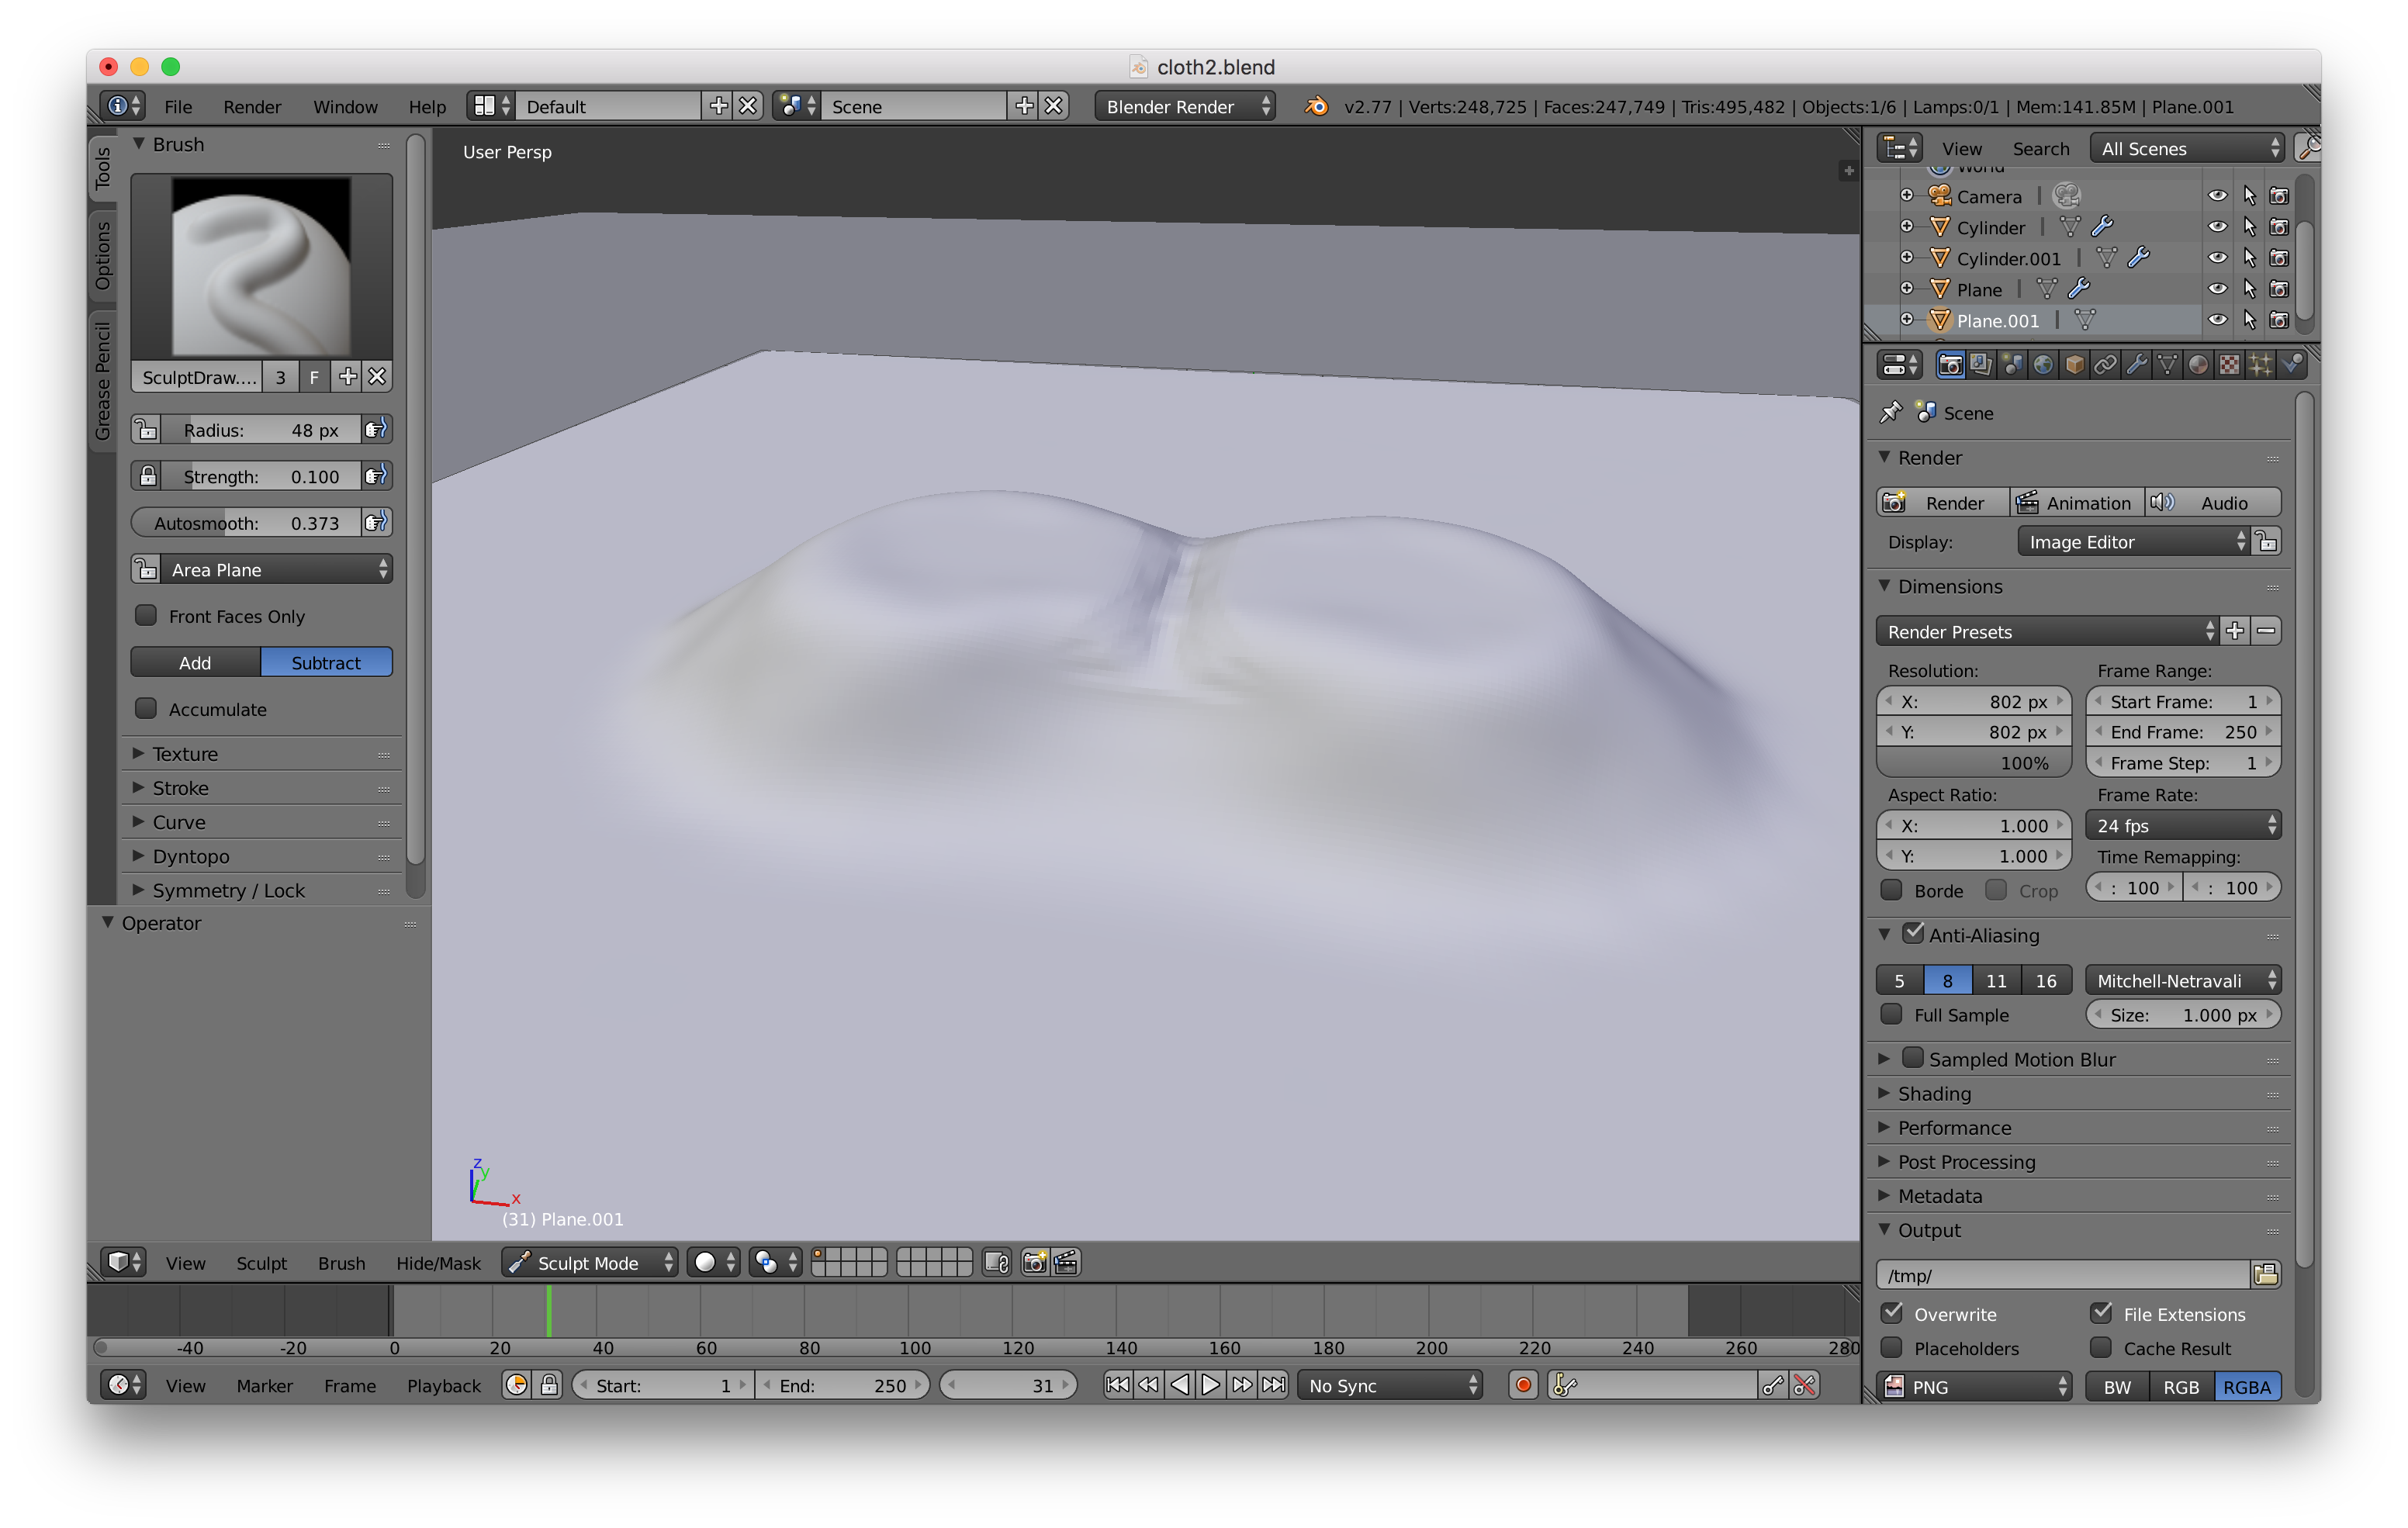
\includegraphics[width=\textwidth]{./images/blender.png}
    \end{subfigure}
  \end{figure*}
\end{abstract}
